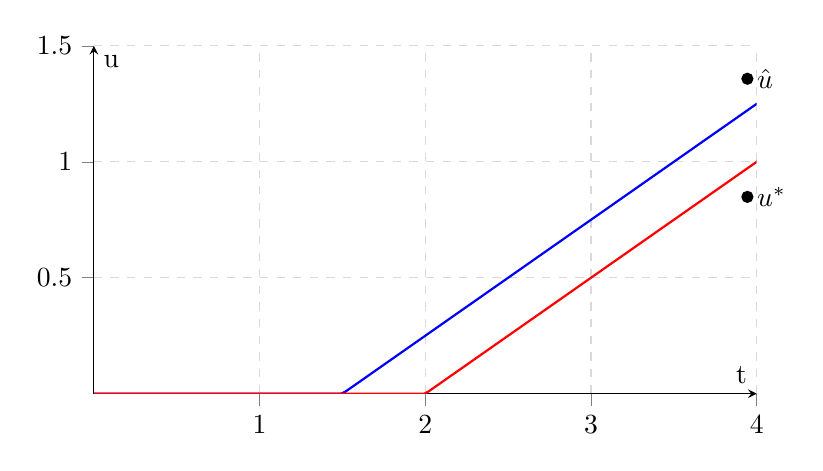
\begin{tikzpicture}[
    declare function={
        f(\x)= (\x <= 1.5) * (0)   +
                  (\x >= 1.5) * (0.5*\x - 0.75)
       ;
       g(\x) =  (\x <=  2) * (0)   +
                  (\x >= 2) * (0.5*\x - 1) 
       ;
      }
    ]
    \begin{axis}[
        axis x line=middle,
        axis y line=middle,
        grid = major,
        width=10cm,
        height=6cm,
        grid style={dashed, gray!30},
        xmin= 0,     % start the diagram at this x-coordinate
        xmax= 4,    % end   the diagram at this x-coordinate
        ymin= 0,     % start the diagram at this y-coordinate
        ymax= 1.5,   % end   the diagram at this y-coordinate
        xlabel=t,
        ylabel=u,
		/pgfplots/xtick={0, 1, ..., 4}, % make steps of length 0.5
		/pgfplots/ytick={0, 0.5, ..., 4}, % make steps of length 0.5
        tick align=outside,
        samples = 400,
        enlargelimits=false]
      % plot the function
	  \addplot [blue,thick] {f(x)};
	  \addplot [red,thick] {g(x)};
    \end{axis}

    \filldraw[black] (8.3,2.5) circle (2pt) node[anchor=west] {$u^*$};
    \filldraw[black] (8.3,4.0) circle (2pt) node[anchor=west] {$\hat{u}$};

\end{tikzpicture}